\documentclass{studentnotes}
\usepackage{graphicx}
\usepackage{subfiles}

% ============================================================
% DOCUMENT INFORMATION
% ============================================================
\setnotetitle{Diffraction and Interference Study Notes}
\setnotecourse{Optics}
\setnoteauthor{Ot}
\setnotedate{\today}

% Uncomment the next line to use the dotted-paper background.
% \usedotgrid

\begin{document}

\makenotetitle%

\tableofcontents
\newpage

% ============================================================
\section{The Central Idea Behind Diffraction}
% ============================================================

Diffraction and interference are governed by one central chain of ideas:

\[
    \boxed{
        \text{Path difference}
        \longrightarrow
        \text{Phase difference}
        \longrightarrow
        \text{Wave addition}
        \longrightarrow
        \text{Intensity}
    }
\]

Suppose two waves travel different distances before arriving at the same observation point. The difference between the distances travelled is called the \textbf{path difference}.

\begin{definition}
    The path difference between two waves is

    \[
        \Delta L=L_2-L_1.
    \]
\end{definition}

A path difference produces a phase difference because one complete wavelength corresponds to one complete phase cycle of \(2\pi\) radians.

\begin{namedformula}{Phase difference}
    \Delta\phi%
    =
    \frac{2\pi}{\lambda}\Delta\,L
\end{namedformula}

Here:

\begin{itemize}
    \item \(\Delta\phi\) is the phase difference;
    \item \(\Delta L\) is the path difference;
    \item \(\lambda\) is the wavelength.
\end{itemize}

\begin{importantnote}
    The geometry of an experiment gives the path difference. The path difference gives the phase difference. The phase difference determines whether waves reinforce or cancel.
\end{importantnote}

\subsection{Constructive and Destructive Interference}

Constructive interference occurs when waves arrive in phase.

\[
    \Delta L=m\lambda,
    \qquad
    m=0,\pm1,\pm2,\ldots
\]

The corresponding phase difference is

\[
    \Delta\phi=2m\pi.
\]

Destructive interference occurs when two waves of equal amplitude arrive exactly out of phase.

\[
    \Delta L=
    \left(m+\frac12\right)\lambda
\]

and therefore

\[
    \Delta\phi=(2m+1)\pi.
\]

\begin{quicknote}
    A path difference of \(\lambda\) returns a wave to the same phase. A path difference of \(\lambda/2\) reverses its phase.
\end{quicknote}

\subsection{Why Diffraction Is an Interference Phenomenon}

In an ordinary two-source interference experiment, two separate sources produce the interfering waves.

In diffraction, different portions of the \emph{same wavefront} act as secondary sources. Waves from different parts of the opening then interfere at the observation point.

Thus,

\[
    \boxed{
        \text{Diffraction is interference involving continuously distributed sources.}
    }
\]

% ============================================================
\section{Single-Slit Diffraction}
% ============================================================

Consider monochromatic light of wavelength \(\lambda\) incident on a slit of width \(a\).

According to the Huygens—Fresnel principle, every point across the slit behaves as a source of secondary waves.

\subsection{Geometry of the Path Difference}

At an observation point making an angle \(\theta\) with the central axis, the ray from one edge of the slit travels farther than the ray from the opposite edge.

\begin{center}
    \fbox{\rule{0.8\textwidth}{0.4\textwidth}}
\end{center}

The total path difference between waves from the top and bottom edges is

\begin{namedformula}{Single-slit path difference}
    \Delta\,L=a\sin\theta%
\end{namedformula}

where:

\begin{itemize}
    \item \(a\) is the slit width;
    \item \(\theta\) is the diffraction angle.
\end{itemize}

\subsection{Condition for Dark Fringes}

The minima of a single-slit diffraction pattern occur when

\begin{namedformula}{Single-slit minima}
    a\sin\theta=m\lambda,
    \qquad
    m=\pm1,\pm2,\pm3,\ldots
\end{namedformula}

The value \(m=0\) is excluded because

\[
    a\sin 0=0
\]

corresponds to the bright central maximum, not a minimum.

Thus:

\[
    \begin{aligned}
        \text{First minimum:}\qquad  & a\sin\theta_1=\lambda,  \\
        \text{Second minimum:}\qquad & a\sin\theta_2=2\lambda, \\
        \text{Third minimum:}\qquad  & a\sin\theta_3=3\lambda.
    \end{aligned}
\]

\subsection{Why the First Minimum Occurs}

For the first minimum,

\[
    a\sin\theta=\lambda.
\]

Divide the slit into two equal halves.

For every source point in the upper half, choose a corresponding source point in the lower half. Their separation is

\[
    \frac{a}{2}.
\]

The path difference between the paired waves is therefore

\[
    \Delta L_{\text{pair}}
    =
    \frac{a}{2}\sin\theta.
\]

Using the first-minimum condition,

\[
    a\sin\theta=\lambda,
\]

we obtain

\[
    \Delta L_{\text{pair}}
    =
    \frac{\lambda}{2}.
\]

This corresponds to a phase difference of

\[
    \Delta\phi
    =
    \frac{2\pi}{\lambda}
    \left(\frac{\lambda}{2}\right)
    =
    \pi.
\]

Therefore, every contribution from one half of the slit is cancelled by a corresponding contribution from the other half.

\[
    \boxed{\text{Resultant amplitude}=0}
\]

and hence

\[
    \boxed{\text{Intensity}=0.}
\]

\begin{personalnote}
    The slit is not dark because waves fail to reach the observation point. It is dark because many waves reach the point and cancel pairwise.
\end{personalnote}

\subsection{Positions of the Minima on a Screen}

Let the screen be a distance \(L\) from the slit. Let the \(m\)-th minimum be a distance \(y_m\) from the central axis.

From the geometry,

\[
    \tan\theta_m=\frac{y_m}{L}.
\]

For small diffraction angles,

\[
    \sin\theta\approx\tan\theta\approx\theta.
\]

Therefore,

\[
    \sin\theta_m\approx\frac{y_m}{L}.
\]

Using

\[
    a\sin\theta_m=m\lambda,
\]

we obtain

\[
    a\left(\frac{y_m}{L}\right)=m\lambda.
\]

Hence,

\begin{namedformula}{Position of single-slit minima}
    y_m=\frac{m\lambda\,L}{a}
\end{namedformula}

\subsection{Width of the Central Maximum}

The central maximum lies between the first minima on either side:

\[
    m=+1
    \qquad\text{and}\qquad
    m=-1.
\]

The first minimum on one side is located at

\[
    y_1=\frac{\lambda L}{a}.
\]

Therefore, the central maximum extends from

\[
    -\frac{\lambda L}{a}
\]

to

\[
    +\frac{\lambda L}{a}.
\]

Its total width is

\begin{namedformula}{Width of central maximum}
    W_{\text{central}}
    =
    \frac{2\lambda\,L}{a}
\end{namedformula}

\subsection{Physical Interpretation}

From

\[
    W_{\text{central}}
    =
    \frac{2\lambda L}{a},
\]

we see that:

\[
    W_{\text{central}}\propto\lambda,
    \qquad
    W_{\text{central}}\propto L,
    \qquad
    W_{\text{central}}\propto\frac{1}{a}.
\]

Therefore:

\begin{itemize}
    \item increasing the wavelength widens the pattern;
    \item increasing the screen distance widens the pattern;
    \item decreasing the slit width widens the pattern;
    \item increasing the slit width narrows the pattern.
\end{itemize}

\begin{importantnote}
    A narrower opening produces greater angular spreading. This inverse relationship between confinement and spreading is one of the deepest ideas in wave physics.
\end{importantnote}

\subsection{Example: Position of the First Minimum}

\begin{example}
    Light of wavelength

    \[
        \lambda=600\,\text{nm}
    \]

    passes through a slit of width

    \[
        a=0.20\,\text{mm}.
    \]

    The screen is

    \[
        L=2.0\,\text{m}
    \]

    away. Find the position of the first minimum.
\end{example}

Convert the quantities to SI units:

\[
    \lambda=600\times10^{-9}\,\text{m},
\]

\[
    a=0.20\times10^{-3}\,\text{m}.
\]

For the first minimum, \(m=1\):

\[
    y_1=\frac{\lambda L}{a}.
\]

Therefore,

\[
    \begin{aligned}
        y_1
         & =
        \frac{(600\times10^{-9})(2.0)}
        {0.20\times10^{-3}} \\
         & =
        6.0\times10^{-3}\,\text{m}.
    \end{aligned}
\]

Thus,

\[
    \boxed{y_1=6.0\,\text{mm}.}
\]

The central maximum has width

\[
    W_{\text{central}}=2y_1=12\,\text{mm}.
\]

% ============================================================
\section{Intensity in Single-Slit Diffraction}
% ============================================================

The minimum condition tells us where the intensity is zero, but it does not describe the brightness at every angle.

The complete single-slit intensity distribution is

\begin{namedformula}{Single-slit intensity}
    I (\theta)
    =
    I_{\max}
    \left(\frac{\sin\beta}{\beta}
    \right)^2
\end{namedformula}

where

\begin{namedformula}{Single-slit phase parameter}
    \beta%
    =
    \frac{\pi\,a\sin\theta}{\lambda}
\end{namedformula}

The function

\[
    \frac{\sin\beta}{\beta}
\]

is related to the sinc function.

\subsection{Meaning of the Parameter \texorpdfstring{\(\beta\)}{beta}}

The total path difference across the slit is

\[
    \Delta L=a\sin\theta.
\]

The corresponding total phase difference is

\[
    \Delta\phi
    =
    \frac{2\pi}{\lambda}\Delta L.
\]

Substituting gives

\[
    \Delta\phi
    =
    \frac{2\pi a\sin\theta}{\lambda}.
\]

The quantity \(\beta\) is defined as half this total phase difference:

\[
    \beta=\frac{\Delta\phi}{2}.
\]

Therefore,

\[
    \boxed{
        \beta=\frac{\pi a\sin\theta}{\lambda}
    }
\]

\begin{quicknote}
    The parameter \(\beta\) is not a new physical angle in space. It is a convenient measure of the phase spread across the slit.
\end{quicknote}

\subsection{Origin of the Factor \texorpdfstring{\(\sin\beta/\beta\)}{sin beta/beta}}

Divide the slit into many very narrow strips.

Each strip contributes a small electric-field amplitude. Because the strips occupy different positions across the slit, their waves reach the observation point with slightly different phases.

These small amplitudes may be represented as phasors.

When the phasors are arranged head-to-tail:

\begin{itemize}
    \item their total arc length represents the amplitude that would occur if all contributions were in phase;
    \item the chord joining the beginning and end of the arc gives the actual resultant amplitude.
\end{itemize}

The geometry of the phasor arc gives

\[
    E(\theta)
    =
    E_{\max}
    \frac{\sin\beta}{\beta}.
\]

Since intensity is proportional to the square of the field amplitude,

\[
    I\propto E^2,
\]

we obtain

\[
    I(\theta)
    =
    I_{\max}
        {\left(
            \frac{\sin\beta}{\beta}
            \right)}^2.
\]

\subsection{Intensity at the Centre}

At the centre,

\[
    \theta=0.
\]

Therefore,

\[
    \beta=0.
\]

The formula appears to contain

\[
    \frac{\sin0}{0}.
\]

However,

\[
    \lim_{\beta\to0}
    \frac{\sin\beta}{\beta}
    =
    1.
\]

Therefore,

\[
    I(0)=I_{\max}.
\]

Thus, the centre is the brightest part of the diffraction pattern.

\subsection{Deriving the Minima from the Intensity Formula}

The intensity is zero when

\[
    \sin\beta=0,
\]

provided \(\beta\neq0\).

Hence,

\[
    \beta=m\pi,
    \qquad
    m=\pm1,\pm2,\ldots
\]

Substitute

\[
    \beta
    =
    \frac{\pi a\sin\theta}{\lambda}:
\]

\[
    \frac{\pi a\sin\theta}{\lambda}=m\pi.
\]

Cancelling \(\pi\),

\[
    a\sin\theta=m\lambda.
\]

Thus, the intensity equation reproduces the single-slit minimum condition.

\subsection{Secondary Maxima}

The secondary maxima occur between consecutive minima.

Starting from

\[
    I(\beta)
    =
    I_{\max}
        {\left(
            \frac{\sin\beta}{\beta}
            \right)}^2,
\]

the condition for a stationary point is

\[
    \frac{dI}{d\beta}=0.
\]

Ignoring the minima where \(\sin\beta=0\), the secondary maxima satisfy

\begin{namedformula}{Secondary-maximum condition}
    \tan\beta=\beta%
\end{namedformula}

The first few nonzero solutions are approximately

\[
    \beta
    \approx
    4.493,\quad
    7.725,\quad
    10.904,\ldots
\]

The first secondary maximum has intensity approximately

\[
    I\approx0.047I_{\max}.
\]

Therefore, it is only about \(4.7\%\) as intense as the central maximum.

\begin{importantnote}
    The central maximum is both wider and much brighter than the secondary maxima.
\end{importantnote}

\subsection{Shape of the Intensity Pattern}

\begin{center}
    \begin{tikzpicture}[xscale=0.75,yscale=4]
        \draw[->] (-7,0) -- (7.4,0) node[right] {\(\beta\)};
        \draw[->] (0,0) -- (0,1.15) node[above] {\(I/I_{\max}\)};

        \draw[domain=-7:7,samples=300,thick,blue]
        plot (\x,{(\x==0) ? 1 : (sin(\x r)/\x)^2});

        \foreach \x in {-6.283,-3.142,3.142,6.283}
        \draw[dashed,gray] (\x,0) -- (\x,0.12);

        \node[below] at (-3.142,0) {\(-\pi\)};
        \node[below] at (3.142,0) {\(\pi\)};
        \node[below] at (6.283,0) {\(2\pi\)};
        \node[below] at (-6.283,0) {\(-2\pi\)};
    \end{tikzpicture}
\end{center}

% ============================================================
\section{Diffraction Through a Circular Aperture}
% ============================================================

Circular apertures occur in:

\begin{itemize}
    \item camera lenses;
    \item telescope mirrors;
    \item microscopes;
    \item the human pupil;
    \item optical instruments.
\end{itemize}

A point source observed through a circular aperture does not form a perfect point image. Instead, it produces a bright central disc surrounded by faint rings.

This diffraction pattern is called the \textbf{Airy pattern}, and the bright central region is called the \textbf{Airy disc}.

\subsection{First Minimum of a Circular Aperture}

For an aperture of diameter \(D\), the first dark ring occurs at

\begin{namedformula}{Circular-aperture first minimum}
    \sin\theta_{\min}
    =
    1.22\frac{\lambda}{D}
\end{namedformula}

For small angles,

\[
    \sin\theta\approx\theta.
\]

Therefore,

\begin{namedformula}{Small-angle circular-aperture formula}
    \theta_{\min}
    \approx%
    1.22\frac{\lambda}{D}
\end{namedformula}

The factor \(1.22\) arises from the circular geometry and the first zero of a Bessel function.

\subsection{Exact Intensity Distribution}

The exact intensity distribution is

\begin{namedformula}{Airy-pattern intensity}
    I (\theta)
    =
    I_{\max}
    \left[
        \frac{2J_1(u)}{u}
        \right]^2
\end{namedformula}

where

\[
    u
    =
    \frac{\pi D\sin\theta}{\lambda}
\]

and \(J_1(u)\) is the Bessel function of the first kind of order one.

The first zero of \(J_1(u)\) occurs near

\[
    u\approx3.8317.
\]

Hence,

\[
    \frac{\pi D\sin\theta}{\lambda}
    \approx3.8317,
\]

so

\[
    \sin\theta
    \approx
    \frac{3.8317}{\pi}
    \frac{\lambda}{D}.
\]

Since

\[
    \frac{3.8317}{\pi}\approx1.22,
\]

we obtain

\[
    \sin\theta_{\min}
    \approx
    1.22\frac{\lambda}{D}.
\]

\subsection{Radius of the Airy Disc}

If a screen is a distance \(L\) away, then

\[
    r=L\tan\theta.
\]

For small angles,

\[
    r\approx L\theta.
\]

Therefore,

\begin{namedformula}{Airy-disc radius}
    r
    =
    1.22\frac{\lambda\,L}{D}
\end{namedformula}

The diameter is

\begin{namedformula}{Airy-disc diameter}
    d_{\text{Airy}}
    =
    2.44\frac{\lambda\,L}{D}
\end{namedformula}

If the pattern is formed in the focal plane of a lens of focal length \(f\), replace \(L\) with \(f\):

\[
    r
    =
    1.22\frac{\lambda f}{D}.
\]

\subsection{Rayleigh Criterion}

Two point sources are said to be \textbf{just resolved} when the central maximum of one Airy pattern lies at the first minimum of the other.

The minimum resolvable angular separation is

\begin{namedformula}{Rayleigh criterion}
    \theta_R
    =
    1.22\frac{\lambda}{D}
\end{namedformula}

\begin{importantnote}
    A smaller value of \(\theta_R\) means better angular resolution.
\end{importantnote}

Since

\[
    \theta_R\propto\frac{\lambda}{D},
\]

resolution improves when:

\begin{itemize}
    \item the aperture diameter is increased;
    \item the wavelength is decreased.
\end{itemize}

\subsection{Example: Telescope Resolution}

\begin{example}
    A telescope has an aperture diameter

    \[
        D=0.20\,\text{m}
    \]

    and observes light of wavelength

    \[
        \lambda=550\,\text{nm}.
    \]

    Find its diffraction-limited angular resolution.
\end{example}

Use

\[
    \theta_R
    =
    1.22\frac{\lambda}{D}.
\]

Thus,

\[
    \begin{aligned}
        \theta_R
         & =
        1.22
        \frac{550\times10^{-9}}{0.20} \\
         & =
        3.36\times10^{-6}\,\text{rad}.
    \end{aligned}
\]

Therefore,

\[
    \boxed{
        \theta_R
        \approx
        3.36\times10^{-6}\,\text{rad}
    }
\]

% ============================================================
\section{Double-Slit Diffraction and Interference}
% ============================================================

For a real double-slit system, define:

\begin{itemize}
    \item \(a\): width of each slit;
    \item \(d\): centre-to-centre slit separation;
    \item \(\lambda\): wavelength;
    \item \(L\): distance to the screen.
\end{itemize}

Two effects occur simultaneously:

\[
    \boxed{
        \text{Each slit diffracts}
        \quad+\quad
        \text{the two slits interfere}
    }
\]

\subsection{Ideal Double Slit}

First suppose each slit is extremely narrow, so diffraction from each slit may be neglected.

The path difference between waves from the two slit centres is

\begin{namedformula}{Double-slit path difference}
    \Delta\,L=d\sin\theta%
\end{namedformula}

The corresponding phase difference is

\[
    \delta
    =
    \frac{2\pi}{\lambda}d\sin\theta.
\]

Define

\begin{namedformula}{Double-slit phase parameter}
    \alpha%
    =
    \frac{\pi\,d\sin\theta}{\lambda}
\end{namedformula}

so that

\[
    \delta=2\alpha.
\]

\subsection{Deriving the Ideal Double-Slit Intensity}

Suppose each slit contributes an electric-field amplitude \(E_0\).

The resultant amplitude of two waves with phase difference \(\delta\) is

\[
    E=2E_0\cos\left(\frac{\delta}{2}\right).
\]

Since

\[
    \frac{\delta}{2}=\alpha,
\]

we have

\[
    E=2E_0\cos\alpha.
\]

Intensity is proportional to the square of amplitude:

\[
    I\propto E^2.
\]

Hence,

\[
    I
    =
    4I_s\cos^2\alpha,
\]

where \(I_s\) is the intensity due to one slit.

If the maximum intensity is defined as

\[
    I_{\max}=4I_s,
\]

then

\begin{namedformula}{Ideal double-slit intensity}
    I (\theta)
    =
    I_{\max}\cos^2\alpha%
\end{namedformula}

or

\[
    I(\theta)
    =
    I_{\max}
    \cos^2
    \left(
    \frac{\pi d\sin\theta}{\lambda}
    \right).
\]

\subsection{Bright Fringes}

Constructive interference occurs when

\[
    \Delta L=m\lambda.
\]

Therefore,

\begin{namedformula}{Double-slit bright fringes}
    d\sin\theta=m\lambda,
    \qquad
    m=0,\pm1,\pm2,\ldots
\end{namedformula}

\subsection{Dark Fringes}

Destructive interference occurs when

\[
    \Delta L
    =
    \left(m+\frac12\right)\lambda.
\]

Therefore,

\begin{namedformula}{Double-slit dark fringes}
    d\sin\theta%
    =
    \left(m+\frac12\right)\lambda%
\end{namedformula}

\subsection{Fringe Positions}

For small angles,

\[
    \sin\theta\approx\frac{y}{L}.
\]

Using the bright-fringe condition,

\[
    d\frac{y_m}{L}=m\lambda.
\]

Therefore,

\begin{namedformula}{Bright-fringe position}
    y_m
    =
    \frac{m\lambda\,L}{d}
\end{namedformula}

\subsection{Fringe Spacing}

The spacing between consecutive bright fringes is

\[
    \Delta y
    =
    y_{m+1}-y_m.
\]

Thus,

\[
    \begin{aligned}
        \Delta y
         & =
        \frac{(m+1)\lambda L}{d}
        -
        \frac{m\lambda L}{d} \\
         & =
        \frac{\lambda L}{d}.
    \end{aligned}
\]

Hence,

\begin{namedformula}{Double-slit fringe spacing}
    \Delta\,y
    =
    \frac{\lambda\,L}{d}
\end{namedformula}

\subsection{Real Double Slit}

A real slit has finite width, so each slit produces its own diffraction pattern.

The two-slit interference fringes are therefore modulated by a single-slit diffraction envelope.

The complete intensity is

\begin{namedformula}{Real double-slit intensity}
    I (\theta)
    =
    I_0
    \left(\frac{\sin\beta}{\beta}
    \right)^2
    \cos^2\alpha%
\end{namedformula}

where

\[
    \beta
    =
    \frac{\pi a\sin\theta}{\lambda}
\]

and

\[
    \alpha
    =
    \frac{\pi d\sin\theta}{\lambda}.
\]

Equivalently, if \(I_s\) is the central intensity from one slit,

\[
    I(\theta)
    =
    4I_s
        {\left(
            \frac{\sin\beta}{\beta}
            \right)}^2
    \cos^2\alpha.
\]

\subsection{Interpretation of the Two Factors}

The factor

\[
    {\left(
        \frac{\sin\beta}{\beta}
        \right)}^2
\]

is the broad single-slit diffraction envelope.

The factor

\[
    \cos^2\alpha
\]

produces the narrow double-slit interference fringes.

Thus,

\[
    \boxed{
        \text{Total pattern}
        =
        \text{diffraction envelope}
        \times
        \text{interference pattern}
    }
\]

\begin{personalnote}
    Think of the interference term as drawing narrow vertical stripes. The diffraction term acts like a large lampshade that controls how bright those stripes are.
\end{personalnote}

\subsection{Missing Orders}

An interference maximum occurs when

\[
    d\sin\theta=m\lambda.
\]

A diffraction minimum occurs when

\[
    a\sin\theta=p\lambda,
    \qquad
    p=1,2,3,\ldots
\]

A bright interference fringe disappears when both conditions occur at the same angle.

Dividing the two equations,

\[
    \frac{d}{a}
    =
    \frac{m}{p}.
\]

Therefore,

\begin{namedformula}{Missing-order condition}
    m=p\frac{d}{a}
\end{namedformula}

\begin{example}
    Suppose

    \[
        d=3a.
    \]

    Then

    \[
        m=3p.
    \]

    Hence, the missing interference orders are

    \[
        m=3,6,9,\ldots
    \]
\end{example}

% ============================================================
\section{Diffraction Gratings}
% ============================================================

A diffraction grating consists of a large number of equally spaced parallel slits.

Let:

\begin{itemize}
    \item \(N\) be the number of illuminated slits;
    \item \(d\) be the centre-to-centre spacing between adjacent slits;
    \item \(a\) be the width of each slit.
\end{itemize}

A grating behaves like a many-source interference system.

\subsection{Grating Equation}

The path difference between waves from adjacent slits is

\[
    \Delta L=d\sin\theta.
\]

All adjacent waves arrive in phase when

\[
    d\sin\theta=m\lambda.
\]

Therefore,

\begin{namedformula}{Diffraction-grating equation}
    d\sin\theta=m\lambda,
    \qquad
    m=0,\pm1,\pm2,\ldots
\end{namedformula}

The integer \(m\) is called the \textbf{diffraction order}.

\subsection{Meaning of the Orders}

For \(m=0\),

\[
    \theta=0,
\]

which gives the central or zeroth-order maximum.

For \(m=1\),

\[
    d\sin\theta_1=\lambda,
\]

which gives the first-order maximum.

For \(m=2\),

\[
    d\sin\theta_2=2\lambda,
\]

which gives the second-order maximum.

\subsection{Grating Spacing and Line Density}

Suppose a grating has \(n_g\) lines per unit length.

Then the spacing between adjacent lines is

\begin{namedformula}{Grating spacing}
    d=\frac{1}{n_g}
\end{namedformula}

\begin{example}
    A grating contains

    \[
        600\,\text{lines/mm}.
    \]

    Then

    \[
        d
        =
        \frac{1}{600}\,\text{mm}.
    \]

    Since

    \[
        1\,\text{mm}=10^{-3}\,\text{m},
    \]

    we obtain

    \[
        d
        =
        \frac{10^{-3}}{600}\,\text{m}.
    \]

    Therefore,

    \[
        \boxed{
            d=1.67\times10^{-6}\,\text{m}.
        }
    \]
\end{example}

\subsection{Maximum Possible Order}

The grating equation gives

\[
    \sin\theta=\frac{m\lambda}{d}.
\]

Since

\[
    |\sin\theta|\leq1,
\]

we require

\[
    \frac{|m|\lambda}{d}\leq1.
\]

Thus,

\[
    |m|\leq\frac{d}{\lambda}.
\]

The maximum possible positive order is

\begin{namedformula}{Maximum grating order}
    m_{\max}
    =
    \left\lfloor%
    \frac{d}{\lambda}
    \right\rfloor%
\end{namedformula}

where \(\lfloor x\rfloor\) means the greatest integer not exceeding \(x\).

\begin{quicknote}
    If \(d/\lambda\) is exactly an integer, the highest mathematical order would occur at \(\theta=90^\circ\), which may not be practically observable.
\end{quicknote}

\subsection{Intensity for \texorpdfstring{\(N\)}{N} Narrow Slits}

For \(N\) equally spaced narrow slits, define

\[
    \alpha
    =
    \frac{\pi d\sin\theta}{\lambda}.
\]

The intensity is

\begin{namedformula}{Many-slit intensity}
    I (\theta)
    =
    I_1
    \left(\frac{\sin\,N\alpha}{\sin\alpha}
    \right)^2
\end{namedformula}

where \(I_1\) is the intensity associated with one slit.

At a principal maximum,

\[
    \alpha=m\pi.
\]

Although direct substitution gives \(0/0\), the limiting value is

\[
    \lim_{\alpha\to m\pi}
    \frac{\sin N\alpha}{\sin\alpha}
    =
    N.
\]

Therefore,

\[
    I_{\max}=N^2I_1.
\]

Thus,

\begin{namedformula}{Principal-maximum intensity}
    I_{\max}\propto\,N^2
\end{namedformula}

\subsection{Why Many Slits Produce Sharp Peaks}

Suppose the phase difference between adjacent slits changes slightly by an amount \(\varepsilon\).

The phase difference between the first and last slit is approximately

\[
    (N-1)\varepsilon.
\]

When \(N\) is large, even a small \(\varepsilon\) produces a large total phase spread.

Consequently, the waves cancel strongly except very close to the principal maxima.

Therefore, increasing \(N\):

\begin{itemize}
    \item makes the principal maxima brighter;
    \item makes them narrower;
    \item improves the ability to distinguish nearby wavelengths.
\end{itemize}

\subsection{Finite Slit Width}

If each grating slit has width \(a\), the full intensity becomes

\begin{namedformula}{Finite-width grating intensity}
    I (\theta)
    =
    I_1
    \left(\frac{\sin\beta}{\beta}
    \right)^2
    \left(\frac{\sin\,N\alpha}{\sin\alpha}
    \right)^2
\end{namedformula}

where

\[
    \beta
    =
    \frac{\pi a\sin\theta}{\lambda}
\]

and

\[
    \alpha
    =
    \frac{\pi d\sin\theta}{\lambda}.
\]

The factor

\[
    {\left(
        \frac{\sin\beta}{\beta}
        \right)}^2
\]

is the single-slit diffraction envelope.

The factor

\[
    {\left(\frac{\sin N\alpha}{\sin\alpha}
        \right)}^2
\]

is the many-slit interference pattern.

\subsection{Angular Width of a Principal Maximum}

The approximate angular width between the neighbouring minima around the \(m\)-th principal maximum is

\begin{namedformula}{Angular width of a grating maximum}
    \Delta\theta%
    \approx%
    \frac{2\lambda}
    {Nd\cos\theta_m}
\end{namedformula}

The half-width is

\[
    \delta\theta
    \approx
    \frac{\lambda}
    {Nd\cos\theta_m}.
\]

Therefore,

\[
    \Delta\theta\propto\frac{1}{N}.
\]

More illuminated slits produce narrower maxima.

\subsection{Angular Dispersion}

The grating equation is

\[
    d\sin\theta=m\lambda.
\]

Differentiate with respect to \(\lambda\), treating \(d\) and \(m\) as constants:

\[
    d\cos\theta\frac{d\theta}{d\lambda}=m.
\]

Therefore,

\begin{namedformula}{Angular dispersion}
    \frac{d\theta}{d\lambda}
    =
    \frac{m}{d\cos\theta}
\end{namedformula}

Angular dispersion increases when:

\begin{itemize}
    \item the order \(m\) increases;
    \item the grating spacing \(d\) decreases;
    \item the diffraction angle increases.
\end{itemize}

\subsection{Resolving Power}

The resolving power of a grating is defined as

\[
    R
    =
    \frac{\lambda}{\Delta\lambda},
\]

where \(\Delta\lambda\) is the smallest wavelength difference that can be resolved.

For a diffraction grating,

\begin{namedformula}{Grating resolving power}
    R
    =
    \frac{\lambda}{\Delta\lambda}
    =
    mN
\end{namedformula}

Therefore,

\begin{namedformula}{Minimum resolvable wavelength difference}
    \Delta\lambda_{\min}
    =
    \frac{\lambda}{mN}
\end{namedformula}

Resolution improves when:

\begin{itemize}
    \item a higher diffraction order is used;
    \item more grating lines are illuminated.
\end{itemize}

\subsection{Example: Grating Angle}

\begin{example}
    Light of wavelength

    \[
        \lambda=500\,\text{nm}
    \]

    is incident on a grating with

    \[
        600\,\text{lines/mm}.
    \]

    Find the first-order diffraction angle.
\end{example}

The grating spacing is

\[
    d
    =
    \frac{10^{-3}}{600}
    =
    1.67\times10^{-6}\,\text{m}.
\]

For the first order, \(m=1\):

\[
    d\sin\theta=\lambda.
\]

Therefore,

\[
    \sin\theta
    =
    \frac{\lambda}{d}.
\]

Substituting,

\[
    \sin\theta
    =
    \frac{500\times10^{-9}}
    {1.67\times10^{-6}}
    \approx0.300.
\]

Hence,

\[
    \boxed{
        \theta\approx17.5^\circ.
    }
\]

% ============================================================
\section{X-Ray Diffraction}
% ============================================================

Visible light has wavelengths of approximately

\[
    \lambda_{\text{visible}}
    \sim
    400\text{--}700\,\text{nm}.
\]

Typical atomic spacings are approximately

\[
    d\sim0.1\,\text{nm}.
\]

Visible light therefore has a wavelength much larger than the spacing between atoms.

X-rays, however, commonly have wavelengths of order

\[
    \lambda_{\text{X-ray}}
    \sim
    10^{-10}\,\text{m},
\]

which is comparable to atomic spacings.

A crystal can therefore act as a three-dimensional diffraction grating for X-rays.

\subsection{Crystal Planes}

Atoms in a crystal may be regarded as lying in sets of parallel planes separated by a distance \(d\).

X-rays incident on these planes are scattered by the atoms.

Strong reflected intensity occurs when the waves scattered from successive planes interfere constructively.

\subsection{Geometry of Bragg Diffraction}

\begin{center}
    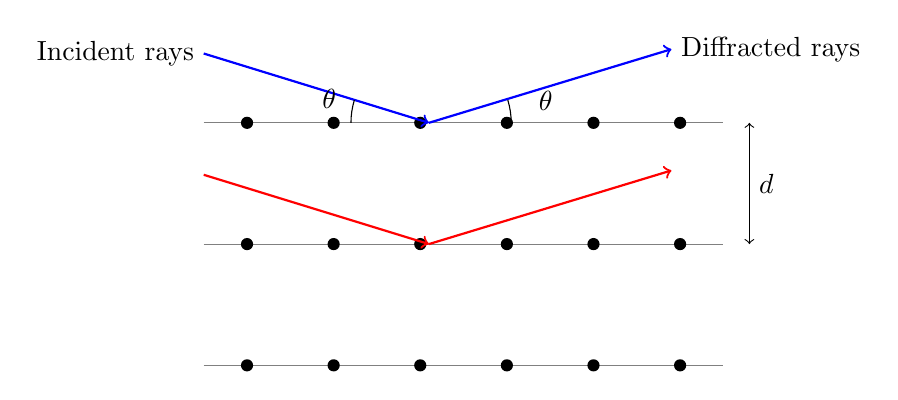
\begin{tikzpicture}[scale=1.1]
        \foreach \y in {0,1.4,2.8}{
                \draw[gray] (-3,\y) -- (3,\y);
                \foreach \x in {-2.5,-1.5,...,2.5}{
                        \fill (\x,\y) circle (2pt);
                    }
            }

        \draw[->,thick,blue] (-3,3.6) -- (-0.4,2.8);
        \draw[->,thick,blue] (-0.4,2.8) -- (2.4,3.65);

        \draw[->,thick,red] (-3,2.2) -- (-0.4,1.4);
        \draw[->,thick,red] (-0.4,1.4) -- (2.4,2.25);

        \draw[<->] (3.3,1.4) -- (3.3,2.8);
        \node[right] at (3.3,2.1) {\(d\)};

        \draw (-1.3,2.8) arc[start angle=180,end angle=163,radius=0.9];
        \node at (-1.55,3.08) {\(\theta\)};

        \draw (0.55,2.8) arc[start angle=0,end angle=17,radius=0.9];
        \node at (0.95,3.05) {\(\theta\)};

        \node[left] at (-3,3.6) {Incident rays};
        \node[right] at (2.4,3.65) {Diffracted rays};
    \end{tikzpicture}
\end{center}

One ray reflects from an upper crystal plane. Another penetrates to the next plane before being reflected.

The second ray travels extra distance on the way into the crystal and again on the way out.

Each extra segment has length

\[
    d\sin\theta.
\]

Therefore, the total path difference is

\[
    \Delta L
    =
    d\sin\theta+d\sin\theta.
\]

Thus,

\begin{namedformula}{Crystal-plane path difference}
    \Delta\,L
    =
    2d\sin\theta%
\end{namedformula}

\subsection{Bragg's Law}

Constructive interference occurs when the path difference is an integer multiple of the wavelength:

\[
    2d\sin\theta=n\lambda.
\]

Therefore,

\begin{namedformula}{Bragg's law}
    n\lambda%
    =
    2d\sin\theta%
\end{namedformula}

where:

\begin{itemize}
    \item \(n=1,2,3,\ldots\) is the diffraction order;
    \item \(\lambda\) is the X-ray wavelength;
    \item \(d\) is the spacing between crystal planes;
    \item \(\theta\) is the Bragg angle.
\end{itemize}

\subsection{Why the Factor of Two Appears}

The deeper ray travels an additional distance twice:

\[
    \text{extra distance entering}
    =
    d\sin\theta,
\]

and

\[
    \text{extra distance leaving}
    =
    d\sin\theta.
\]

Therefore,

\[
    \Delta L
    =
    d\sin\theta+d\sin\theta
    =
    2d\sin\theta.
\]

\subsection{The \texorpdfstring{\(2\theta\)}{2\theta} Convention}

In many X-ray diffraction instruments, the angle displayed by the detector is the angle between the incident and diffracted beams.

This angle is

\[
    2\theta.
\]

However, Bragg's law uses \(\theta\):

\[
    n\lambda=2d\sin\theta.
\]

\begin{importantnote}
    If an X-ray diffraction problem gives the measured scattering angle as \(2\theta\), divide it by two before substituting into Bragg's law.
\end{importantnote}

\subsection{Example: Finding Crystal-Plane Spacing}

\begin{example}
    X-rays of wavelength

    \[
        \lambda=0.154\,\text{nm}
    \]

    produce a first-order Bragg peak at

    \[
        \theta=30^\circ.
    \]

    Find the spacing between the crystal planes.
\end{example}

For first order,

\[
    n=1.
\]

Bragg's law gives

\[
    n\lambda
    =
    2d\sin\theta.
\]

Therefore,

\[
    d
    =
    \frac{n\lambda}{2\sin\theta}.
\]

Substituting,

\[
    d
    =
    \frac{0.154}
    {2\sin30^\circ}
    \,\text{nm}.
\]

Since

\[
    \sin30^\circ=\frac12,
\]

we obtain

\[
    d
    =
    \frac{0.154}{1}
    \,\text{nm}.
\]

Thus,

\[
    \boxed{
        d=0.154\,\text{nm}.
    }
\]

\subsection{Uses of X-Ray Diffraction}

X-ray diffraction can be used to determine:

\begin{itemize}
    \item crystal-plane spacings;
    \item crystal structures;
    \item lattice constants;
    \item material phases;
    \item molecular arrangements;
    \item strain and defects in crystalline materials.
\end{itemize}

% ============================================================
\section{Comparison of the Main Formulas}
% ============================================================

\begin{center}
    \renewcommand{\arraystretch}{1.5}
    \begin{tabular}{
            >{\raggedright\arraybackslash}p{3.1cm}
            >{\centering\arraybackslash}p{2.7cm}
            >{\centering\arraybackslash}p{4.3cm}
            >{\raggedright\arraybackslash}p{3.2cm}
        }
        \toprule
        \textbf{Arrangement}
         &
        \textbf{Important dimension}
         &
        \textbf{Main formula}
         &
        \textbf{What it locates}
        \\
        \midrule

        Single slit
         &
        Slit width \(a\)
         &
        \(a\sin\theta=m\lambda\)
         &
        Dark minima
        \\

        Double slit
         &
        Slit separation \(d\)
         &
        \(d\sin\theta=m\lambda\)
         &
        Bright fringes
        \\

        Diffraction grating
         &
        Grating spacing \(d\)
         &
        \(d\sin\theta=m\lambda\)
         &
        Principal maxima
        \\

        Circular aperture
         &
        Diameter \(D\)
         &
        \(\theta_{\min}=1.22\lambda/D\)
         &
        First dark ring
        \\

        Crystal planes
         &
        Plane spacing \(d\)
         &
        \(n\lambda=2d\sin\theta\)
         &
        X-ray diffraction maxima
        \\

        \bottomrule
    \end{tabular}
\end{center}

\subsection{The Most Important Distinction}

For a single slit,

\[
    \boxed{
        a\sin\theta=m\lambda
        \quad\text{locates minima.}
    }
\]

For a double slit or diffraction grating,

\[
    \boxed{
        d\sin\theta=m\lambda
        \quad\text{locates maxima.}
    }
\]

The equations look similar, but they describe different features of the patterns.

\begin{remembernote}
    Single slit: integer wavelengths give darkness.

    Double slit and grating: integer wavelengths give brightness.
\end{remembernote}

% ============================================================
\section{Problem-Solving Strategy}
% ============================================================

When solving a diffraction problem, use the following method.

\subsection{Step 1: Identify the Arrangement}

Ask whether the problem involves:

\begin{itemize}
    \item one slit;
    \item two slits;
    \item many slits;
    \item a circular aperture;
    \item crystal planes.
\end{itemize}

\subsection{Step 2: Identify the Relevant Dimension}

Determine whether the important dimension is:

\begin{itemize}
    \item slit width \(a\);
    \item slit separation \(d\);
    \item aperture diameter \(D\);
    \item crystal-plane spacing \(d\).
\end{itemize}

\subsection{Step 3: Identify What Is Being Requested}

Determine whether the problem asks for:

\begin{itemize}
    \item a minimum;
    \item a maximum;
    \item fringe position;
    \item fringe spacing;
    \item central-maximum width;
    \item angular resolution;
    \item grating order;
    \item crystal spacing;
    \item intensity.
\end{itemize}

\subsection{Step 4: Choose the Correct Equation}

Use:

\[
    a\sin\theta=m\lambda
\]

for single-slit minima;

\[
    d\sin\theta=m\lambda
\]

for double-slit or grating maxima;

\[
    \theta_R=1.22\frac{\lambda}{D}
\]

for circular-aperture resolution;

\[
    n\lambda=2d\sin\theta
\]

for X-ray diffraction.

\subsection{Step 5: Check the Angle Convention}

For screen-position problems, use

\[
    \tan\theta=\frac{y}{L}.
\]

For small angles,

\[
    \sin\theta\approx\tan\theta\approx\frac{y}{L}.
\]

For X-ray diffraction, check whether the stated angle is \(\theta\) or \(2\theta\).

\subsection{Step 6: Convert All Units}

Common conversions include

\[
    1\,\text{nm}=10^{-9}\,\text{m},
\]

\[
    1\,\mu\text{m}=10^{-6}\,\text{m},
\]

\[
    1\,\text{mm}=10^{-3}\,\text{m}.
\]

\subsection{Step 7: Check Physical Possibility}

For grating problems,

\[
    |\sin\theta|\leq1.
\]

Therefore, a calculated value such as

\[
    \sin\theta=1.4
\]

means that the proposed diffraction order does not exist.

% ============================================================
\section{Common Mistakes}
% ============================================================

\begin{enumerate}
    \item Using the single-slit minimum formula as though it located bright fringes.

    \item Confusing slit width \(a\) with slit separation \(d\).

    \item Forgetting that a real double slit contains both diffraction and interference.

    \item Using line density directly as the grating spacing instead of taking its reciprocal.

    \item Forgetting to convert lines per millimetre into lines per metre.

    \item Using the full measured X-ray angle \(2\theta\) in Bragg's law.

    \item Using small-angle approximations when the angle is not small.

    \item Including \(m=0\) as a single-slit minimum.

    \item Forgetting that intensity is proportional to the square of amplitude.

    \item Assuming that narrower slits produce narrower diffraction patterns.
\end{enumerate}

% ============================================================
\section{Formula Sheet}
% ============================================================

\subsection{General Phase Relation}

\[
    \boxed{
        \Delta\phi
        =
        \frac{2\pi}{\lambda}\Delta L
    }
\]

\subsection{Single Slit}

\[
    \boxed{
        a\sin\theta=m\lambda
    }
    \qquad
    \text{minima}
\]

\[
    \boxed{
        y_m
        =
        \frac{m\lambda L}{a}
    }
\]

\[
    \boxed{
        W_{\text{central}}
        =
        \frac{2\lambda L}{a}
    }
\]

\[
    \boxed{
        I(\theta)
        =
        I_{\max}
            {\left(
                \frac{\sin\beta}{\beta}
                \right)}^2
    }
\]

\[
    \boxed{
        \beta
        =
        \frac{\pi a\sin\theta}{\lambda}
    }
\]

\[
    \boxed{
        \tan\beta=\beta
    }
    \qquad
    \text{secondary maxima}
\]

\subsection{Circular Aperture}

\[
    \boxed{
        \theta_{\min}
        =
        1.22\frac{\lambda}{D}
    }
\]

\[
    \boxed{
        r
        =
        1.22\frac{\lambda L}{D}
    }
\]

\[
    \boxed{
        d_{\text{Airy}}
        =
        2.44\frac{\lambda L}{D}
    }
\]

\[
    \boxed{
        \theta_R
        =
        1.22\frac{\lambda}{D}
    }
\]

\subsection{Double Slit}

\[
    \boxed{
        d\sin\theta=m\lambda
    }
    \qquad
    \text{bright fringes}
\]

\[
    \boxed{
        d\sin\theta
        =
        \left(m+\frac12\right)\lambda
    }
    \qquad
    \text{dark fringes}
\]

\[
    \boxed{
        y_m
        =
        \frac{m\lambda L}{d}
    }
\]

\[
    \boxed{
        \Delta y
        =
        \frac{\lambda L}{d}
    }
\]

\[
    \boxed{
        I
        =
        I_{\max}\cos^2\alpha
    }
\]

\[
    \boxed{
        \alpha
        =
        \frac{\pi d\sin\theta}{\lambda}
    }
\]

\[
    \boxed{
        I
        =
        I_0
            {\left(
                \frac{\sin\beta}{\beta}
                \right)}^2
        \cos^2\alpha
    }
\]

\subsection{Diffraction Grating}

\[
    \boxed{
        d\sin\theta=m\lambda
    }
\]

\[
    \boxed{
        d=\frac{1}{n_g}
    }
\]

\[
    \boxed{
        m_{\max}
        =
        \left\lfloor
        \frac{d}{\lambda}
        \right\rfloor
    }
\]

\[
    \boxed{
        I
        =
        I_1
            {\left(
                \frac{\sin N\alpha}{\sin\alpha}
                \right)}^2
    }
\]

\[
    \boxed{
        \Delta\theta
        \approx
        \frac{2\lambda}
        {Nd\cos\theta_m}
    }
\]

\[
    \boxed{
        \frac{d\theta}{d\lambda}
        =
        \frac{m}{d\cos\theta}
    }
\]

\[
    \boxed{
        R
        =
        \frac{\lambda}{\Delta\lambda}
        =
        mN
    }
\]

\subsection{X-Ray Diffraction}

\[
    \boxed{
        \Delta L
        =
        2d\sin\theta
    }
\]

\[
    \boxed{
        n\lambda
        =
        2d\sin\theta
    }
\]

% ============================================================
\section{Final Conceptual Map}
% ============================================================

Every diffraction formula follows the same reasoning:

\[
    \boxed{
        \begin{array}{c}
            \text{Identify the contributing waves}
            \\[0.4em]
            \downarrow
            \\[0.4em]
            \text{Find their path difference}
            \\[0.4em]
            \downarrow
            \\[0.4em]
            \text{Convert it into phase difference}
            \\[0.4em]
            \downarrow
            \\[0.4em]
            \text{Add the wave amplitudes}
            \\[0.4em]
            \downarrow
            \\[0.4em]
            \text{Square the resultant amplitude to obtain intensity}
        \end{array}
    }
\]

The physical systems differ, but the logic remains the same:

\[
    \boxed{
        \text{Geometry determines phase, and phase determines brightness.}
    }
\]

\end{document}
